\section{Point-spread function and aperture coupling}
\label{sec:psf}

The point-spread function is the currency in which three different
questions are paid: how much of a star's light enters a photometric
aperture of a given radius, how much passes a slit of a given width and
decentring, and how much lands on the single brightest pixel (the
saturation question). All three are integrals of the same profile over
different domains, and all three are sensitive to the profile's
\emph{wings}: real seeing profiles carry far more energy at large radii
than a Gaussian of the same FWHM, which makes Gaussian-based aperture
corrections optimistic and Gaussian-based saturation predictions
slightly pessimistic. \spetc{} therefore offers both the Gaussian (for
comparability with other tools) and the Moffat profile (for realism),
everywhere through analytic expressions --- no PSF is ever rendered or
numerically integrated, which keeps the whole-night time series fast.

The seeing-limited PSF is selectable between a circular Gaussian and a
circular \citet{moffat1969} profile
\begin{equation}
  I(r) \propto \Big(1 + \frac{r^2}{\alpha^2}\Big)^{-\beta},
  \qquad
  \alpha = \frac{\rm FWHM}{2\sqrt{2^{1/\beta}-1}},
\end{equation}
whose power-law wings ($\beta \simeq 2.5$--$4.7$; the Gaussian is the
$\beta\to\infty$ limit) reproduce real seeing profiles that a Gaussian
underestimates.

\paragraph{Encircled energy.} For a circular aperture of radius $r$,
\begin{equation}
  \mathrm{EE}_{\rm Gauss}(r) = 1 - e^{-r^2/2\sigma^2},
  \qquad
  \mathrm{EE}_{\rm Moffat}(r) = 1 - \Big(1+\frac{r^2}{\alpha^2}\Big)^{1-\beta}.
\end{equation}

\paragraph{Slit coupling.} The flux through an infinite slit of width $w$
whose centre is displaced by $\delta$ from the PSF centroid uses the
one-dimensional marginal profile. For the Gaussian this is the usual error
function; for the circular Moffat the marginal is \emph{exactly} a Student-$t$
distribution with $\nu = 2\beta-2$ degrees of freedom and scale
$\alpha/\sqrt{\nu}$, so
\begin{equation}
  T(w,\delta) \;=\;
  F_\nu\!\Big(\frac{w/2-\delta}{\alpha/\sqrt{\nu}}\Big) -
  F_\nu\!\Big(\frac{-w/2-\delta}{\alpha/\sqrt{\nu}}\Big),
  \label{eq:slit}
\end{equation}
with $F_\nu$ the Student-$t$ CDF --- no numerical integration is required.
The same expression with $w$ equal to one pixel gives the central-pixel
fraction used for saturation prediction, as the separable product of the
dispersion and spatial couplings. Figure~\ref{fig:psf} compares the models.

\begin{figure}
  \centering
  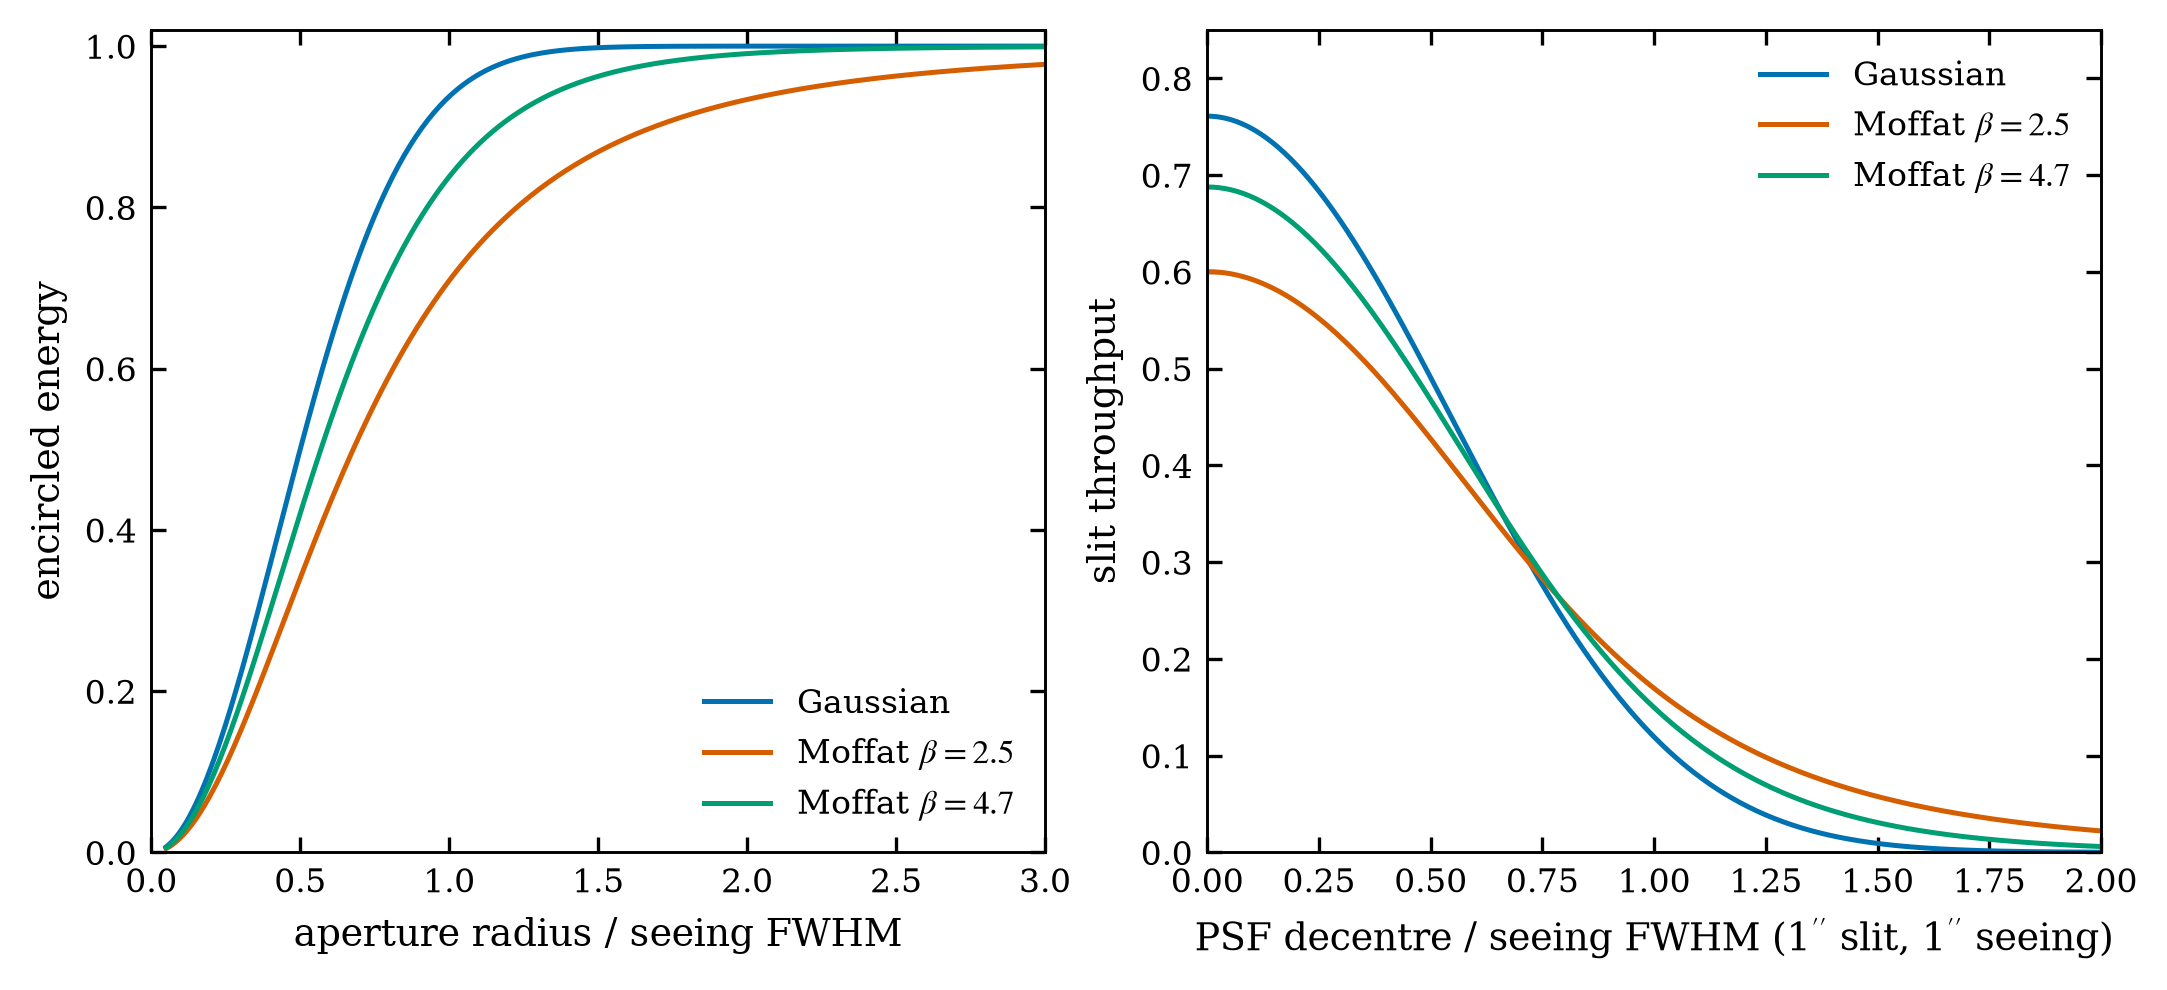
\includegraphics[width=\textwidth]{figures/fig_03_psf.png}
  \caption{Left: encircled energy versus aperture radius in units of the
  seeing FWHM. Right: slit throughput of a slit of one seeing-FWHM width as
  the PSF is decentred, Eq.~(\ref{eq:slit}); the Moffat wings both lower the
  centred coupling and soften the decentring penalty.}
  \label{fig:psf}
\end{figure}

\subsection{Wavelength and airmass dependence of the seeing}
\label{sec:seeing-scaling}

The seeing FWHM is not a constant of the night: Kolmogorov turbulence gives
a Fried parameter $r_0 \propto \lambda^{6/5}(\cos z)^{3/5}$ and hence a
seeing FWHM $\propto \lambda/r_0$,
\begin{equation}
  \mathrm{FWHM}(\lambda, X) \;=\; s_{V,\rm zenith}\;
  X^{0.6}\;\Big(\frac{\lambda}{5000\,\text{\AA}}\Big)^{-0.2},
  \label{eq:seeing-scaling}
\end{equation}
where $s_{V,\rm zenith}$ is the entered zenith seeing in $V$ and $X$ the
airmass. This is the exact form used by ETC-42
\citep[CeSAM/LAM,][\code{calculator/psf/Seeing.java}]{etc42}. As an
optional mode, \spetc{} applies Eq.~(\ref{eq:seeing-scaling}) per wavelength
in the spectroscopic slit and extraction couplings (so blue light suffers
larger losses than red through the same slit), and at the observing band's
pivot wavelength in photometry. Because the airmass factor is evaluated per
time sample, the whole-night time series then correctly shows the seeing ---
and the losses that follow from it --- degrading as the target sets. The
mode is off by default, leaving the seeing flat; when it is on, the entered
value is by definition the zenith $V$ seeing.

\subsection{Guiding blur}
\label{sec:guiding}

Over a long exposure the star also moves: periodic error, polar-alignment
drift and guiding corrections smear the image. If the tracking error is
approximately Gaussian with rms $\sigma_g$ per axis, the time-averaged
image is the seeing profile convolved with a Gaussian of FWHM
$2.355\,\sigma_g$, and the effective image width entering every coupling
of this section is
\begin{equation}
  \mathrm{FWHM}_{\rm eff} \;=\;
  \sqrt{\mathrm{FWHM}_{\rm seeing}^2 + (2.355\,\sigma_g)^2}.
\end{equation}
An entered guiding rms of 0 (the default) reproduces the pure-seeing
case; a typical unguided minute on a mid-range mount
($\sigma_g \sim 1''$) visibly lowers aperture and slit couplings, which
is exactly the effect amateurs observe between guided and unguided
frames (v10.2).

\subsection{Defocused PSF: the geometric donut}
\label{sec:defocus}

Defocused photometry spreads a bright star deliberately over many pixels to
suppress scintillation, flat-field residuals and saturation. When the
detector is displaced by a distance $\delta$ from the focal plane, the
geometric image of a point source is the projection of the (annular) pupil:
a uniformly-illuminated ring, or ``donut''. For a primary of diameter $D$
and focal length $F$ (focal ratio $N = F/D$), similar triangles give a blur
circle of full diameter $\delta/N = \delta D/F$, i.e.\ an outer radius on the
focal plane
\begin{equation}
  r_{\rm out} \;=\; \frac{\delta D}{2F},
\end{equation}
which depends only on $|\delta|$: intra- and extra-focal displacements of
equal magnitude give identical images. A central obstruction of linear
fraction $\varepsilon = D_{\rm obs}/D$ (a classical Ritchey--Chr\'etien or
Cassegrain, $\varepsilon>0$) blocks the inner cone and leaves a hole of
radius $r_{\rm in} = \varepsilon\,r_{\rm out}$; a classical reflector modelled
with $\varepsilon = 0$ gives a filled disc. A uniformly illuminated pupil maps,
in the geometric limit, to a flat annulus, so the encircled energy is analytic:
\begin{equation}
  \mathrm{EE}(r) \;=\;
  \begin{cases}
    0, & r < r_{\rm in},\\[2pt]
    \dfrac{r^2 - r_{\rm in}^2}{r_{\rm out}^2 - r_{\rm in}^2}, & r_{\rm in} \le r \le r_{\rm out},\\[8pt]
    1, & r > r_{\rm out}.
  \end{cases}
\end{equation}
Focal-plane radii convert to angle through the plate scale
($\SI{1}{\micro\metre} \to 206264.8\times10^{-3}/F_{\rm mm}$ arcsec) and to
pixels through the pixel pitch. The user selects a photometry aperture radius
$r_{\rm ap}$ from this curve; the captured light fraction is
$\mathrm{EE}(r_{\rm ap})$, and the peak pixel holds the uniform annulus
surface brightness $L_{\rm tot}/[\pi(r_{\rm out}^2 - r_{\rm in}^2)]$ times the
pixel solid angle --- orders of magnitude below the focused stellar peak,
which is the whole benefit of defocusing.

This is a geometric-optics model: it omits diffraction ringing at the donut
edges, optical aberrations (small on-axis for a paraboloid or an RC) and the
seeing that convolves and softens the rim, all negligible once the donut is
much larger than the seeing and diffraction scales --- the regime in which
defocused photometry operates.
